\documentclass{ximera}

%% You can put user macros here
%% However, you cannot make new environments

\listfiles

\graphicspath{{./}{firstExample/}{secondExample/}}

\usepackage{tikz}
\usepackage{tkz-euclide}
\usepackage{tikz-3dplot}
\usepackage{tikz-cd}
\usetikzlibrary{shapes.geometric}
\usetikzlibrary{arrows}
\usetikzlibrary{decorations.pathmorphing,patterns}
\usetkzobj{all}
\pgfplotsset{compat=1.13} % prevents compile error.

\renewcommand{\vec}[1]{\mathbf{#1}}
\newcommand{\RR}{\mathbb{R}}
\newcommand{\dfn}{\textit}
\newcommand{\dotp}{\cdot}
\newcommand{\id}{\text{id}}
\newcommand\norm[1]{\left\lVert#1\right\rVert}
 
\newtheorem{general}{Generalization}
\newtheorem{initprob}{Exploration Problem}

\tikzstyle geometryDiagrams=[ultra thick,color=blue!50!black]

\usepackage{mathtools}

\title{Newton's Second Law of Motion}


\begin{document}

\begin{abstract}

\end{abstract}

\maketitle



\section*{Newton's Second Law of Motion}


In this section we consider an object with constant mass $m$ moving
along a line under a force $F$. Let $y=y(t)$ be the displacement of
the object from a reference point on the line at time $t$, and let
$v=v(t)$ and $a=a(t)$ be the velocity and acceleration of the object
at time $t$. Thus, $v=y'$ and $a=v'=y''$, where the prime denotes
differentiation with respect to $t$. Newton's second law of motion
asserts that the force $F$ and the acceleration $a$ are related by the
equation
\begin{equation} \label{eq:4.3.1}
F=ma.
\end{equation}

\subsection*{Units}

In applications there are three main sets of units in use for length,
mass, force, and time: the cgs, mks, and British systems. All three
use the second as the unit of time. Table~1 shows the other units.
 Consistent with (\ref{eq:4.3.1}), the unit of
force in each system is defined to be the force required to impart an
acceleration of (one unit of length)$/s^2$ to one unit of
mass.

\bigskip
\begin{center}
\begin{tabular}{|c|c|c|c|}
\hline
& {\bf Length}&{\bf Force}& {\bf Mass}\\\hline
  cgs & centimeter (cm) & dyne (d) & gram (g)\\\hline
 mks & meter (m) & newton (N) & kilogram (kg) \\\hline
British & foot (ft) & pound (lb) & slug (sl)\\\hline
\end{tabular}

Table 1.
\end{center}

If we assume that Earth is a perfect sphere with constant mass
density,  Newton's law of gravitation (discussed later in this
section) asserts that the force exerted on an object by Earth's
gravitational field is proportional to the mass of the object and
inversely proportional to the square of its  distance from the
center of Earth. However, if the object remains sufficiently close to
Earth's surface, we may assume that the gravitational force is
constant and equal to its value at the surface. The magnitude of this
force is $mg$, where $g$ is called the \textit{acceleration due to
gravity}. (To be completely accurate, $g$ should be called the \textit{magnitude of the acceleration due to gravity at Earth's surface}.)
This quantity has been determined experimentally. Approximate
values of $g$  are
$$\begin{array}{rl}
g &=980\ \mbox{cm/s}^2\quad \mbox{(cgs)}   \\
g &=9.8\ \mbox{m/s}^2\quad \mbox{(mks)}   \\
g &=32\ \mbox{ft/s}^2\quad \mbox{(British)}
\end{array}$$

In general, the force $F$ in (\ref{eq:4.3.1}) may depend upon $t$, $y$, and
$y'$. Since $a=y''$,  (\ref{eq:4.3.1}) can be written in the
form
\begin{equation} \label{eq:4.3.2}
my''=F(t,y,y'),
\end{equation}
which is a second order equation. We'll consider this equation with
restrictions on $F$ later;     however, since earlier we have
dealt only with first order equations, we consider here only problems in
which (\ref{eq:4.3.2}) can be recast as a first order equation. This is
possible if $F$ does not depend on $y$, so (\ref{eq:4.3.2}) is of the form
$$
my''=F(t,y').
$$
 Letting $v=y'$ and $v'=y''$ yields a first order
equation for $v$:
\begin{equation} \label{eq:4.3.3}
mv'=F(t,v).
\end{equation}
Solving this equation yields $v$ as a function of $t$. If we know
$y(t_0)$ for some time $t_0$, we can  integrate $v$ to obtain $y$
as a function of $t$.

Equations of the form (\ref{eq:4.3.3}) occur in problems involving motion
through a resisting medium.



\subsection*{Motion Through a Resisting Medium Under Constant
Gravitational Force}

Now we consider an object moving vertically in some medium. We assume
that the only forces acting on the object are gravity and resistance
from the medium. We also assume that the motion takes place close to
Earth's surface and take the upward direction to be positive, so
 the gravitational force can be assumed to have the constant value
 $-mg$. We'll see that, under reasonable assumptions on the
resisting force, the velocity approaches a limit as $t\to\infty$.
We call this limit the \textit{terminal velocity}.

\begin{example}\label{example:4.3.1}
An object with mass $m$ moves under constant gravitational force
through a medium that exerts a resistance with magnitude proportional
to the speed of the object. (Recall that the speed of an object is
$|v|$, the absolute value of its velocity $v$.) Find the velocity of
the object as a function of $t$, and find the terminal velocity.
Assume  that the initial velocity is $v_0$.
 

\begin{explanation}
The total force acting on the object is
\begin{equation} \label{eq:4.3.4}
F=-mg+F_1,
\end{equation}
where $-mg$ is  the force due to  gravity and $F_1$ is the
resisting force of the medium, which has magnitude $k|v|$, where $k$ is a
positive constant. If the
object is moving downward ($v\leq 0$),  the resisting force is
upward, as shown in the figure. 

\begin{image}
  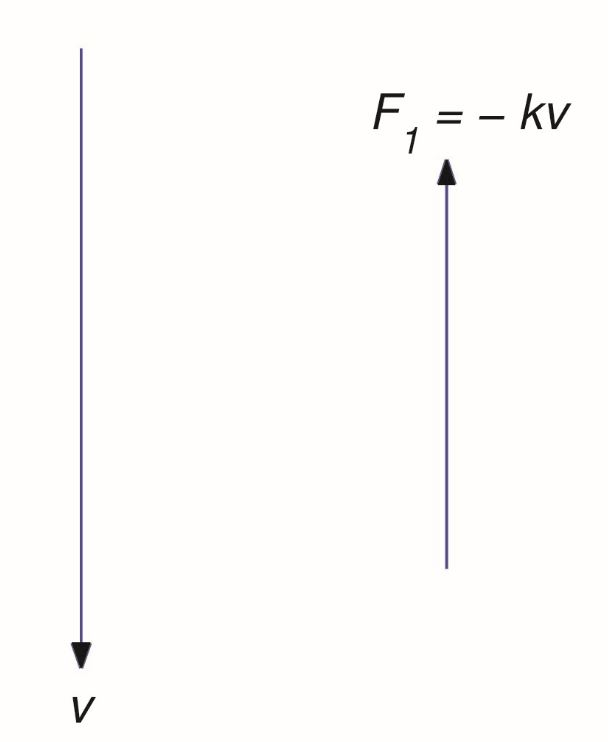
\includegraphics[height=1in]{fig040301a.jpg} 
\end{image}

So
$$
F_1=k|v|=k(-v)=-kv.
$$
On the other hand, if the object is moving upward ($v\geq 0$),
the resisting force is downward, as shown. 

\begin{image}
  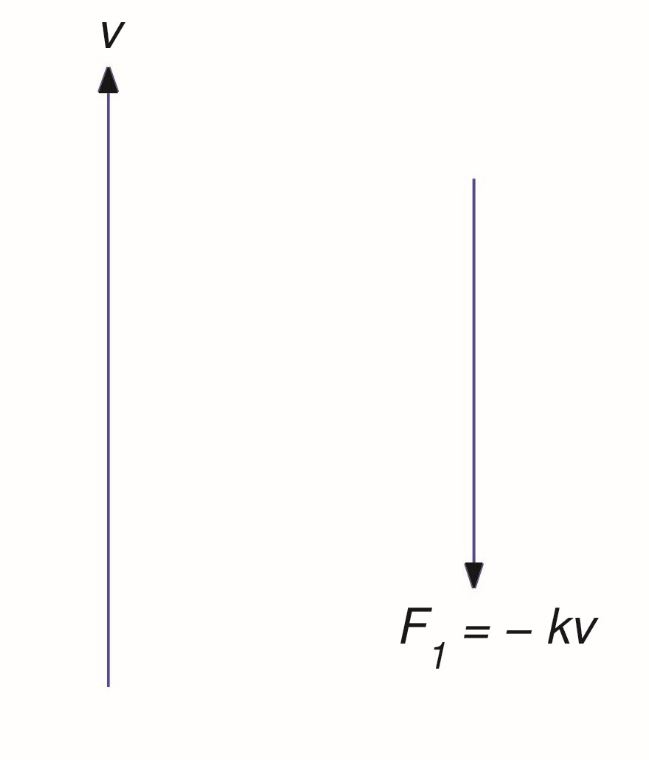
\includegraphics[height=1in]{fig040301b.jpg} 
\end{image}

So
$$
F_1=-k|v|=-kv.
$$
Thus, (\ref{eq:4.3.4}) can be written as
\begin{equation} \label{eq:4.3.5}
F=-mg-kv,
\end{equation}
regardless of the sign of the velocity.

From Newton's second law of motion,
$$
F=ma=mv',
$$
 so (\ref{eq:4.3.5}) yields
$$
mv'=-mg-kv,
$$
 or
\begin{equation} \label{eq:4.3.6}
v'+\frac{k}{m}v=-g.
\end{equation}
Since $e^{-kt/m}$ is a solution of the  complementary
equation, the solutions of (\ref{eq:4.3.6}) are of the form
$v=ue^{-kt/m}$, where $u'e^{-kt/m}=-g$, so $u'=-ge^{kt/m}$.
Hence,
$$
u=-\frac{mg}{k} e^{kt/m}+c,
$$
so
\begin{equation} \label{eq:4.3.7}
v=ue^{-kt/m}=-\frac{mg}{k}+ce^{-kt/m}.
\end{equation}
Since
 $v(0)=v_0$,
$$
v_0=-\frac{mg}{k}+c,
$$
 so
$$
c=v_0+\frac{mg}{k}
$$
 and (\ref{eq:4.3.7}) becomes
$$
v=-\frac{mg}{k}+\left(v_0+\frac{mg}{k}\right) e^{-kt/m}.
$$
Letting $t\rightarrow\infty$ here shows that the terminal velocity is
$$
\lim_{t\rightarrow\infty} v(t)=-\frac{mg}{k},
$$
which  is independent of the
initial velocity $v_0$ (See figure below).

\begin{image}
  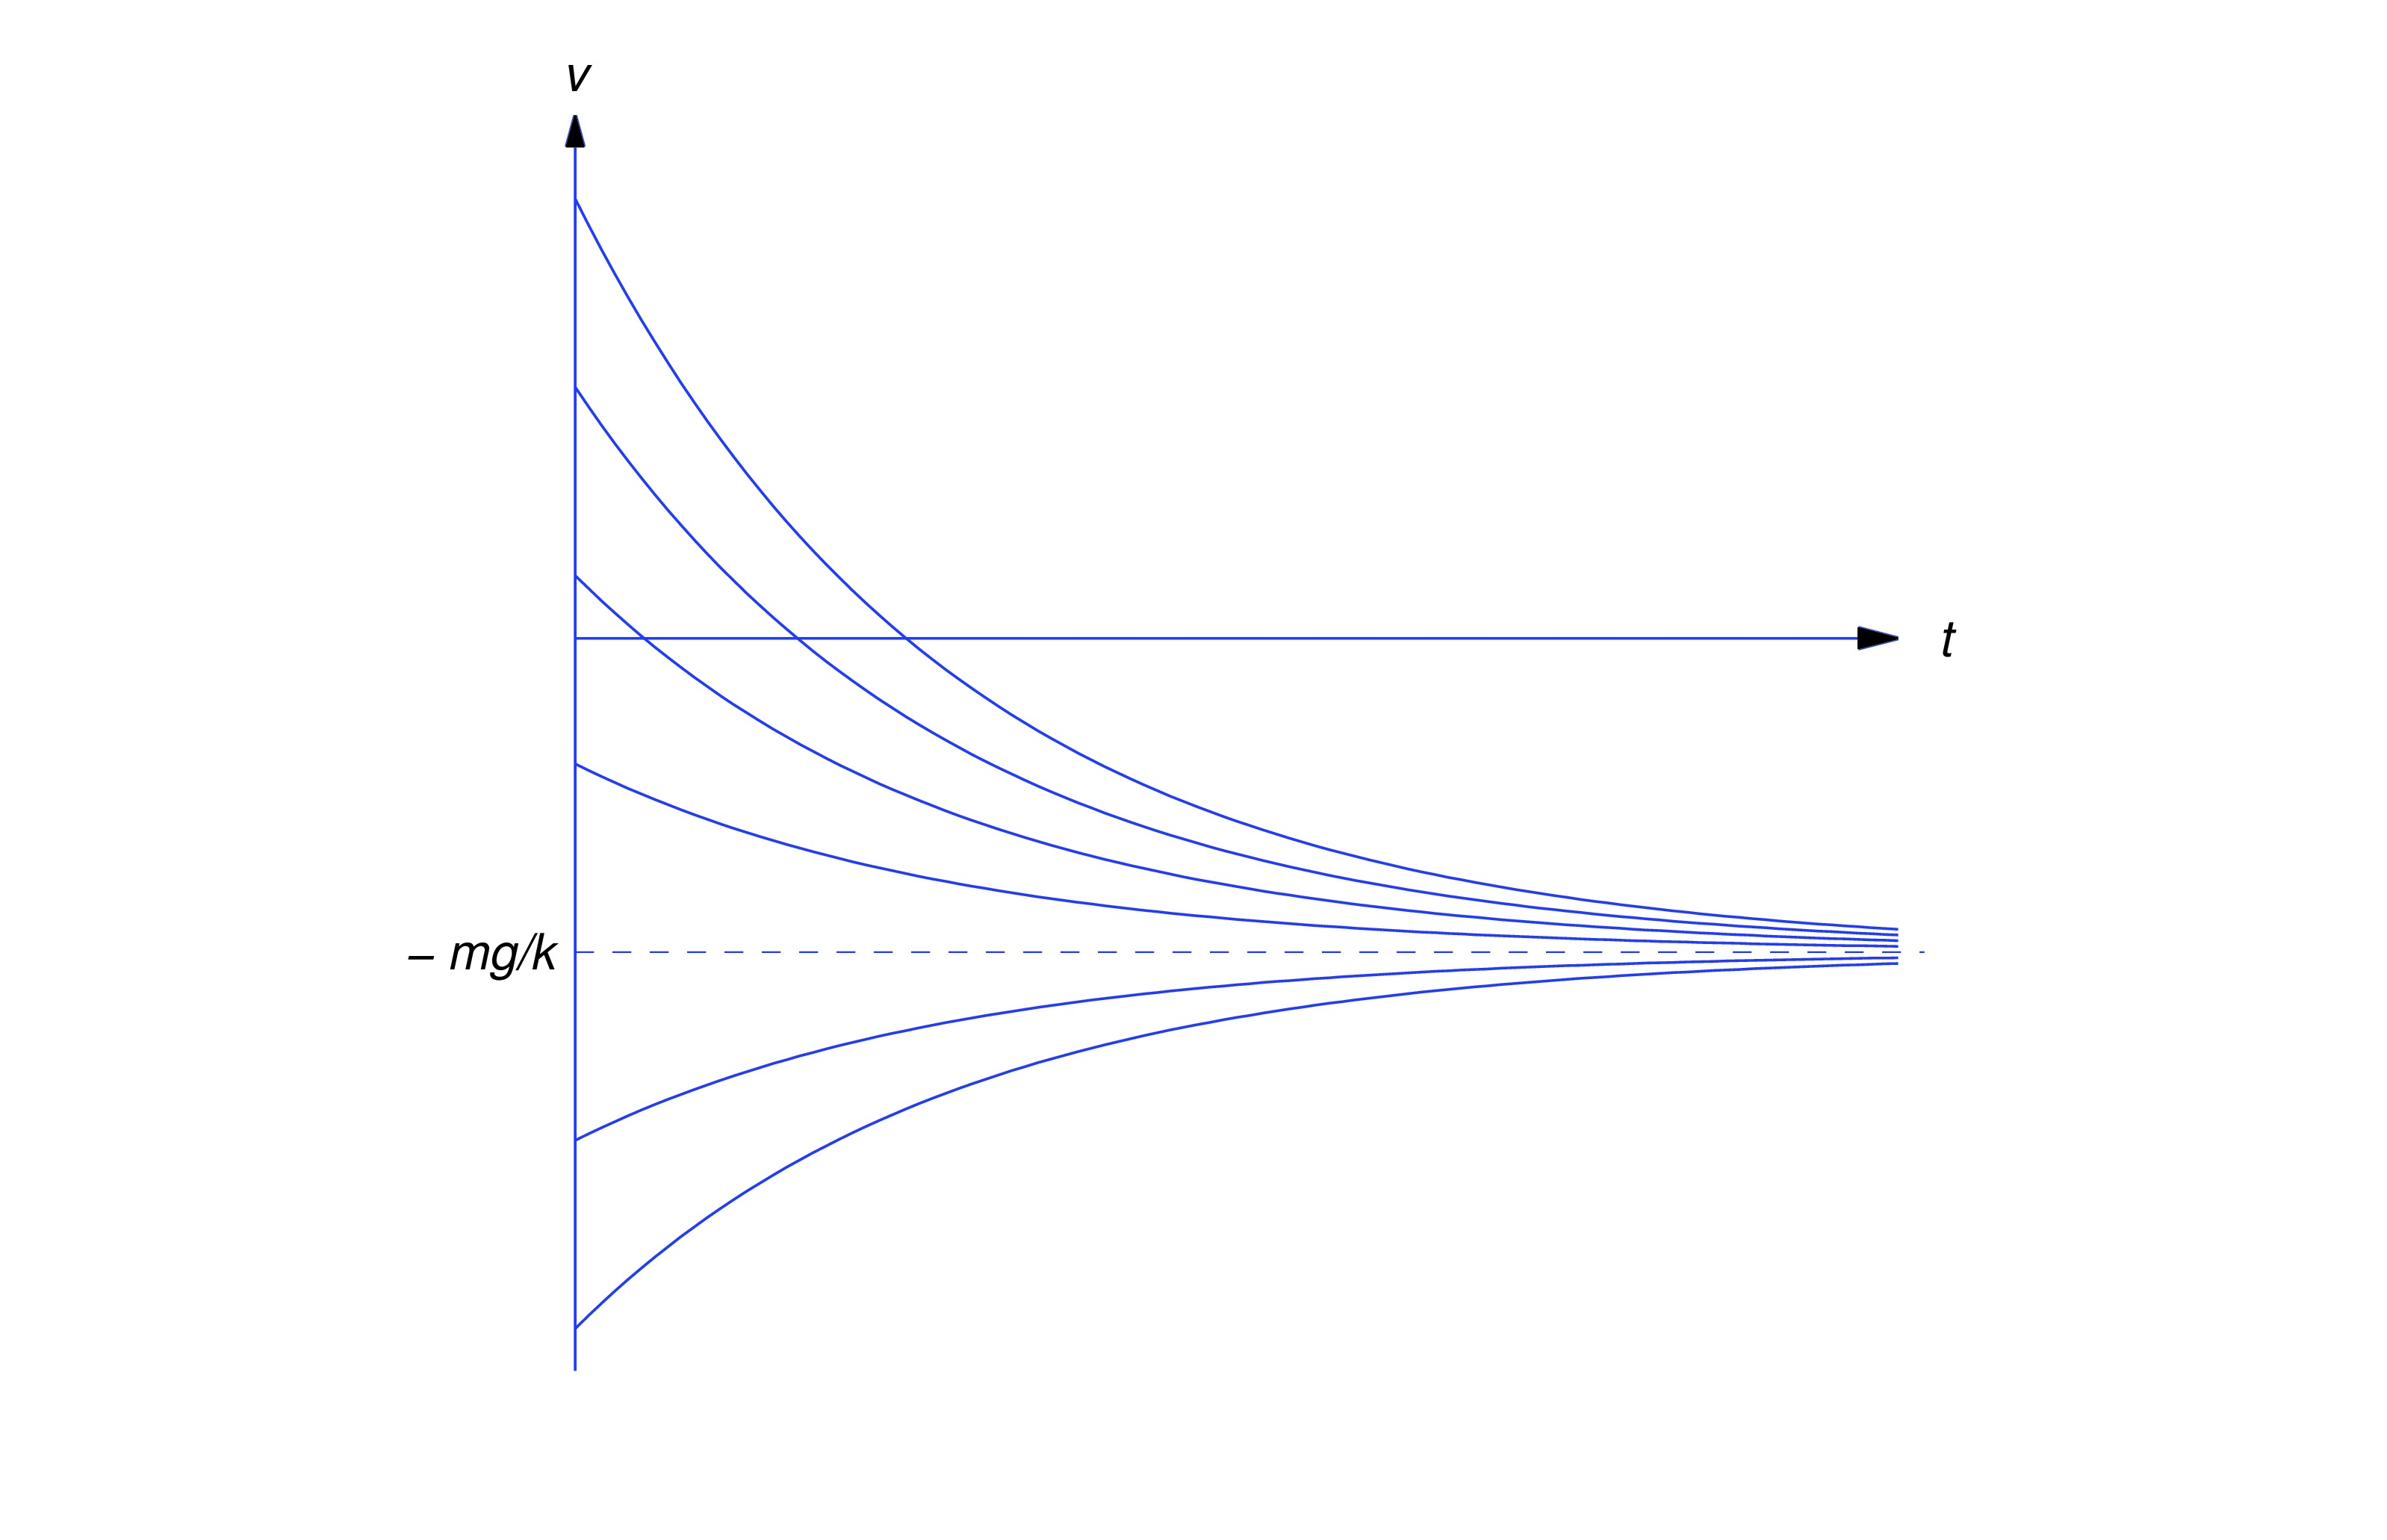
\includegraphics[height=1.5in]{fig040302.jpg} 
\end{image}

\end{explanation}
\end{example}

\begin{example}\label{example:4.3.2}
A 960-lb object is given an initial upward velocity of 60 ft/s near
the surface of Earth. The atmosphere resists the motion with a force
of 3 lb for each ft/s of speed. Assuming that the only other force
acting on the object is constant gravity, find its velocity $v$ as a
function of $t$, and find its  terminal velocity.

\begin{explanation}
Since $mg=960$ and $g=32$,   $m=960/32=30$.  The atmospheric
resistance is $-3v$  lb if $v$ is expressed in feet
per second.  Therefore
$$
30v'=-960-3v,
$$
which we rewrite as
$$
v'+\frac{1}{10}v=-32.
$$
Since $e^{-t/10}$ is a solution of the complementary equation, the
solutions of this equation are of the form $v=ue^{-t/10}$, where
$u'e^{-t/10}=-32$, so $u'=-32e^{t/10}$. Hence,
$$
u=-320 e^{t/10}+c,
$$
so
\begin{equation} \label{eq:4.3.8}
v=ue^{-t/10}=-320+ce^{-t/10}.
\end{equation}
The initial velocity is 60 ft/s in the upward (positive) direction;
hence, $v_0=60$. Substituting $t=0$ and $v=60$ in (\ref{eq:4.3.8})
yields
$$
60=-320+c,
$$
 so $c=380$, and (\ref{eq:4.3.8}) becomes
$$
v=-320+380e^{-t/10}\ \mbox{ft/s}
$$
The terminal velocity is
$$
\lim_{t\to\infty}v(t)=-320\mbox{ ft/s.}
$$
\end{explanation}
\end{example}

\begin{example}\label{example:4.3.3}
A 10 kg mass is given an initial velocity $v_0\leq 0$
 near Earth's surface. The only forces acting on it are
gravity and atmospheric resistance proportional to the square of the
speed. Assuming that the resistance is 8 N if the speed is 2 m/s,
find the velocity of the object as a function of $t$, and
find the terminal velocity.

\begin{explanation} Since the object is falling, the resistance is in the upward
(positive) direction. Hence,
\begin{equation} \label{eq:4.3.9}
mv'=-mg+kv^2,
\end{equation}
where $k$ is a constant. Since the magnitude of the resistance is 8 N
when $v=2$ m/s,
$$
k(2^2)=8,
$$
 so $k=2\  \mbox{N-s}^2/\mbox{m}^2$.  Since
$m=10$ and $g=9.8$, (\ref{eq:4.3.9}) becomes
\begin{equation} \label{eq:4.3.10}
10v'=-98+2v^2=2(v^2-49).
\end{equation}
If $v_0=-7$, then $v\equiv-7$ for all $t\geq 0$. If $v_0\neq -7$,
we separate  variables to obtain
\begin{equation} \label{eq:4.3.11}
\frac{1}{v^2-49}v'=\frac{1}{5},
\end{equation}
which is convenient for the required partial fraction expansion
\begin{equation} \label{eq:4.3.12}
\frac{1}{v^2-49} =\frac{1}{(v-7)(v+7)}
=\frac{1}{14}\left[\frac{1}{v-7}
-\frac{1}{v+7}\right].
\end{equation}
 Substituting (\ref{eq:4.3.12})  into (\ref{eq:4.3.11}) yields
$$
\frac{1}{14}\left[\frac{1}{v-7}-\frac{1}{v+7}\right]v'=\frac{1}{5},
$$
 so
$$
\left[\frac{1}{v-7}-\frac{1}{v+7}\right]v'=\frac{14}{5}.
$$
Integrating this yields
$$
\ln |v-7|-\ln|v+7|=14t/5+k.
$$
Therefore
$$
\left|\frac{v-7}{v+7}\right|=e^ke^{14t/5}.
$$
Since  Theorem~\ref{thmtype:2.3.1}  implies  that  $(v-7)/(v+7)$   can't
change sign (why?), we can rewrite the last equation as
 \begin{equation} \label{eq:4.3.13}
 \frac{v-7}{v+7}=ce^{14t/5},
\end{equation}
which is an implicit solution of (\ref{eq:4.3.10}).
Solving this for $v$ yields
\begin{equation} \label{eq:4.3.14}
v=-7\frac{c+e^{-14t/5}}{c-e^{-14t/5}}.
\end{equation}
 Since $v(0)=v_0$, it
 (\ref{eq:4.3.13}) implies that
$$
c=\frac{v_0-7}{v_0+7}.
$$
 Substituting this into (\ref{eq:4.3.14}) and simplifying yields
$$
v=-7\frac{v_0(1+e^{-14t/5})-7(1-e^{-14t/5})}{v_0(1-e^{-14t/5})-7(1+e^{-14t/5}}.
$$
Since $v_0\leq 0$, $v$ is defined and negative for all
$t>0$. The terminal velocity is
$$
\lim_{t\to\infty} v(t)=-7\  \mbox{m/s},
$$
independent of $v_0$. More generally, it
can be shown (Exercise~\ref{exer:4.3.11}) that if $v$ is any solution
of (\ref{eq:4.3.9}) such that $v_0\leq 0$ then
$$
\lim_{t\to\infty}v(t)=-\sqrt{\frac{mg}{k}}
$$
(See figure below).

\begin{image}
  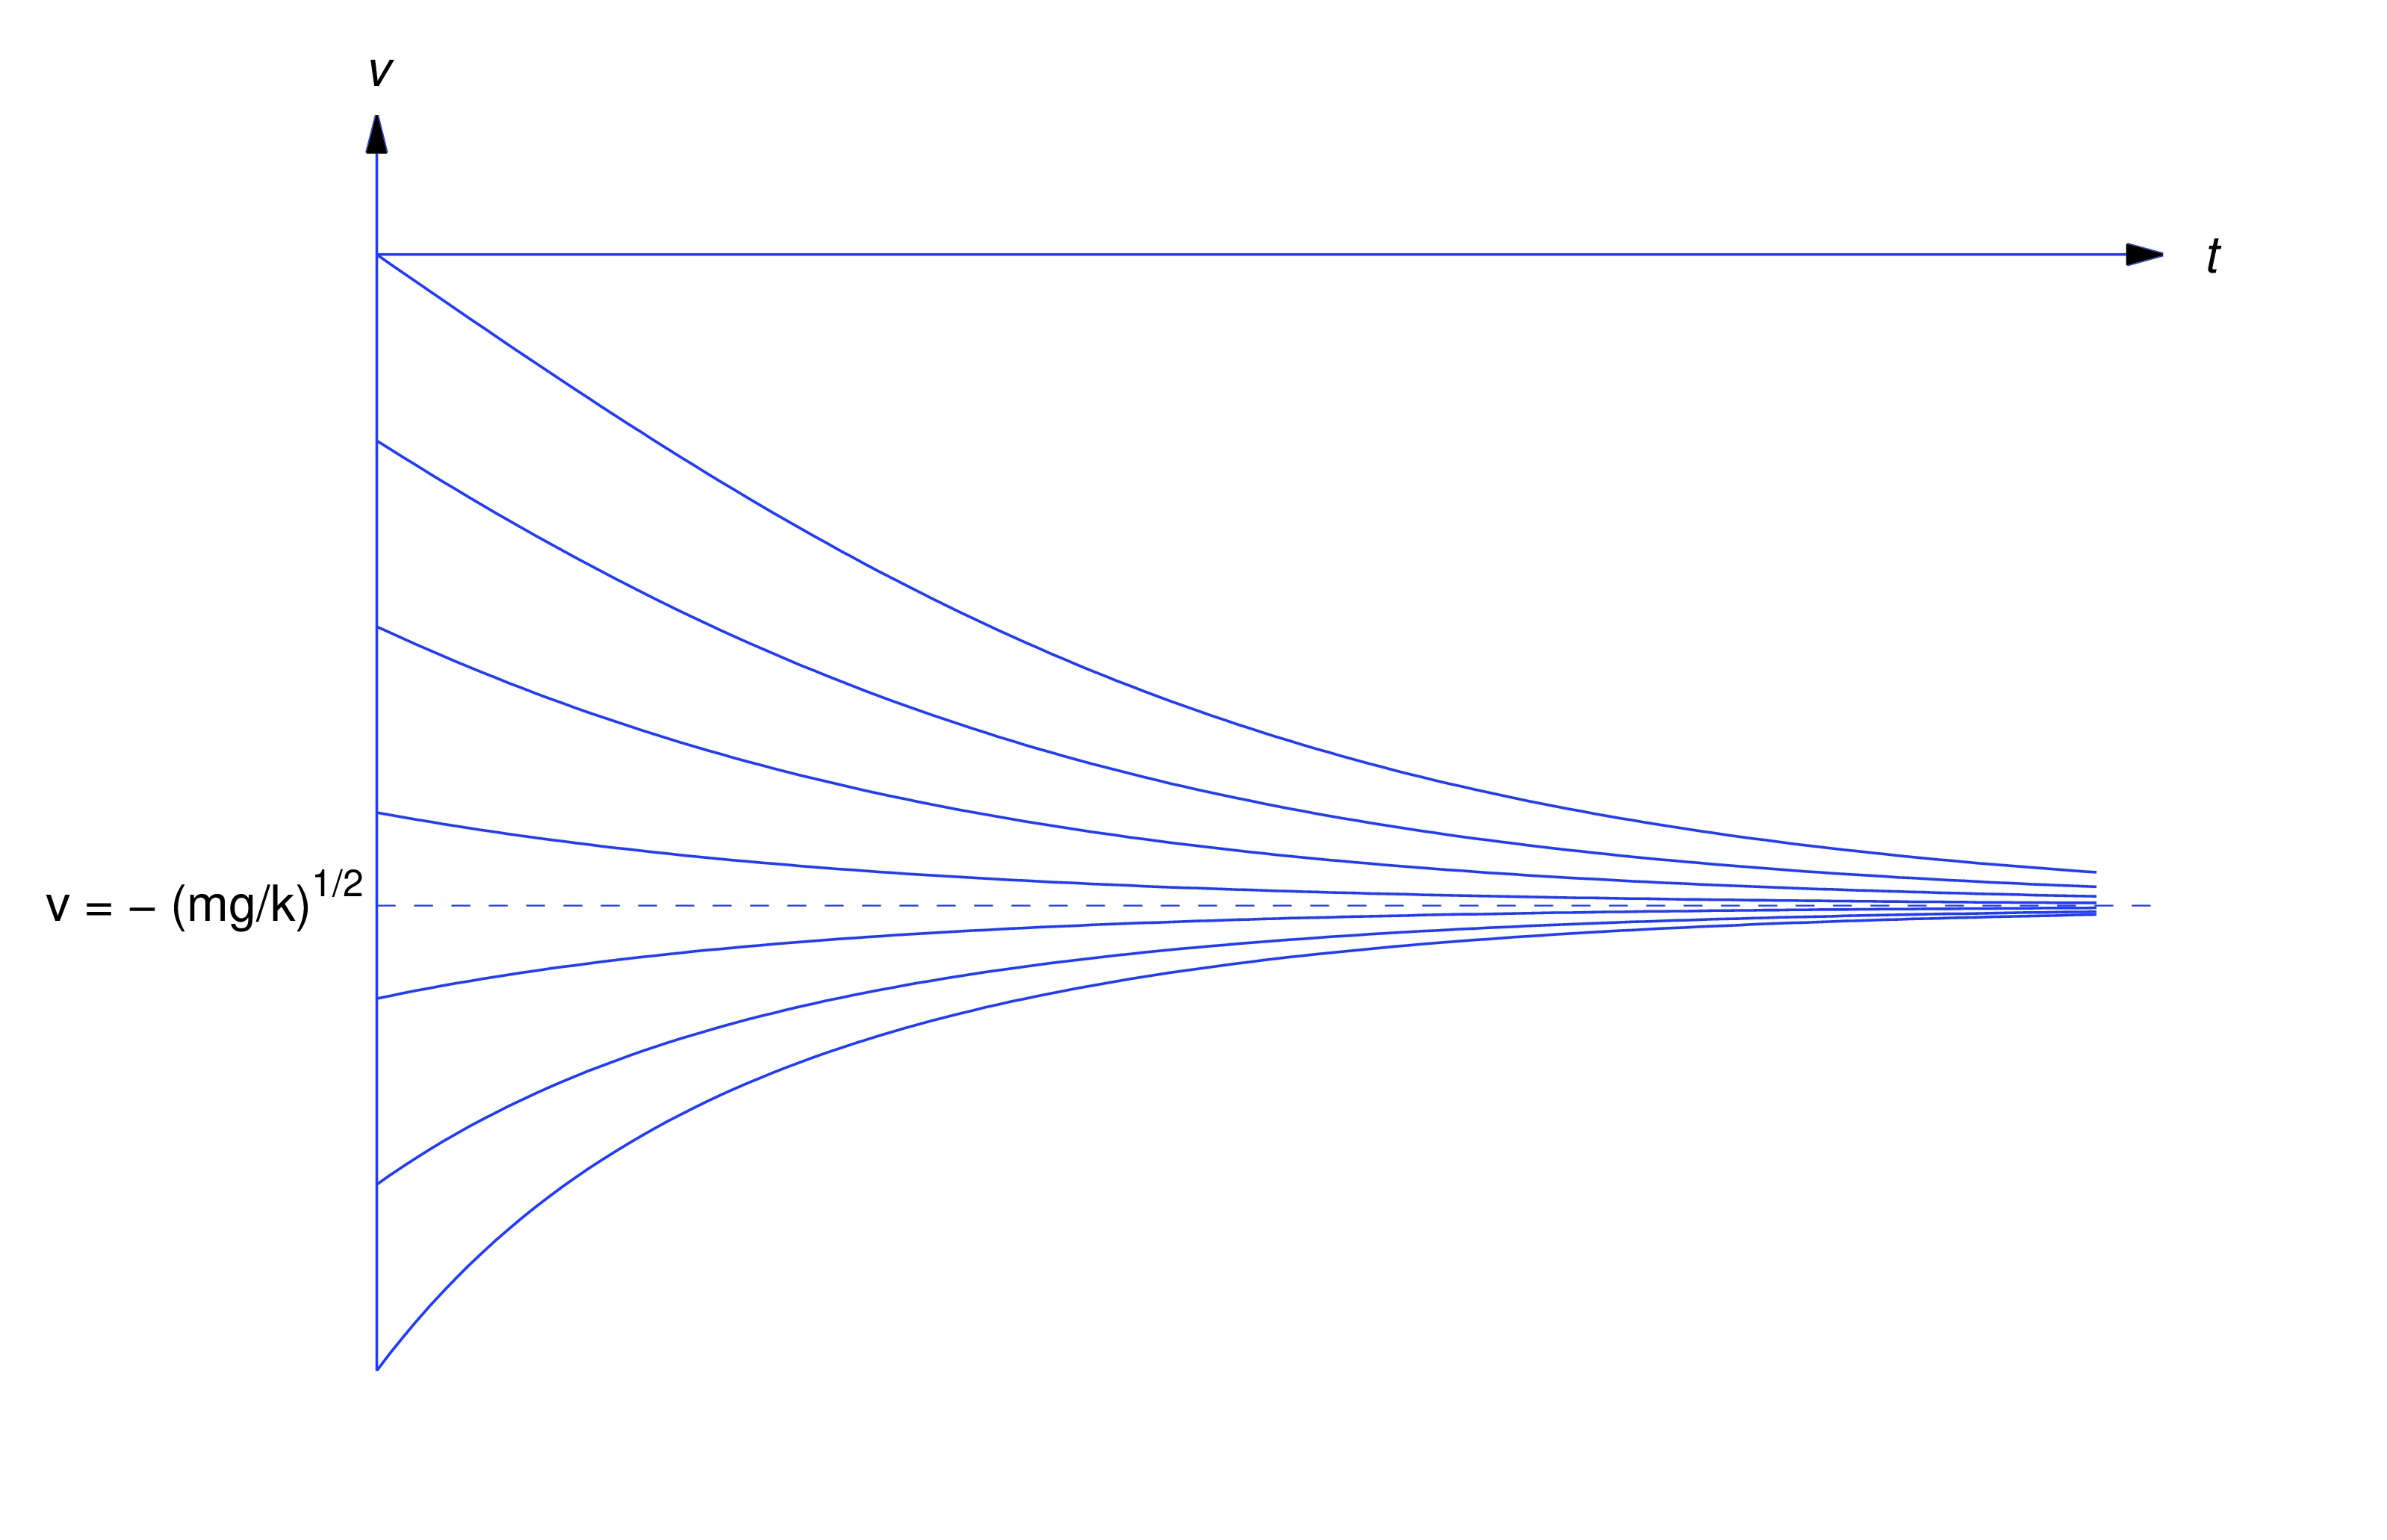
\includegraphics[height=1.5in]{fig040303.jpg} 
\end{image}
\end{explanation}
\end{example}

\begin{example}\label{example:4.3.4}
A 10-kg mass is launched vertically upward from Earth's surface with
an initial velocity of $v_0$ m/s. The only forces acting on the mass
are gravity and atmospheric resistance proportional to the square of
the speed. Assuming that the atmospheric resistance is 8 N if the
speed is 2 m/s, find the time $T$ required for the mass to reach
maximum altitude.


\begin{explanation}  The mass will
climb while $v>0 $ and reach its maximum altitude when $v=0$.
Therefore $v>0$ for $0\leq t<T$ and $v(T)=0$. Although the mass of
the object and our assumptions concerning the forces acting on it are
the same as those in Example \ref{example:4.3.3},  (\ref{eq:4.3.10}) does
not apply here, since the resisting force is negative if $v>0$;
therefore, we replace (\ref{eq:4.3.10}) by
\begin{equation} \label{eq:4.3.15}
10v'=-98-2v^2.
\end{equation}

Separating variables  yields
$$
\frac{5}{v^2+49}v'=-1,
$$
 and integrating this yields
$$
\frac{5}{7}\tan^{-1}\frac{v}{7}=-t+c.
$$
 (Recall that $\tan^{-1}u$ is the number $\theta$
such that $-\pi/2 < \theta < \pi/2$ and $\tan \theta=u$.)
 Since $v(0)=v_0$,
$$
c=\frac{5}{7}\tan^{-1}\frac{v_0}{7},
$$
so $v$ is defined implicitly by
\begin{equation} \label{eq:4.3.16}
\frac{5}{7} \tan^{-1}\frac{v}{7}=-t+\frac{5}{7}
\tan^{-1}\frac{v_0}{7}, \quad 0\leq t\leq T.
\end{equation}
Solving this for $v$ yields
\begin{equation} \label{eq:4.3.17}
v=7\tan\left(-\frac{7t}{5}+\tan^{-1}\frac{v_0}{7}\right).
\end{equation}
Using the identity
$$
\tan(A-B)=\frac{\tan A-\tan B}{1+\tan A\tan B}
$$
with $A=\tan^{-1}(v_0/7)$ and $B=7t/5$, and noting that
$\tan(\tan^{-1}\theta)=\theta$,
we can simplify (\ref{eq:4.3.17}) to
$$
v=7\frac{v_0-7\tan(7t/5)}{7+v_0\tan(7t/5)}.
$$

 Since $v(T)=0$ and $\tan^{-1}(0)=0$, (\ref{eq:4.3.16}) implies that
$$
-T+\frac{5}{7} \tan^{-1}\frac{v_0}{7}=0.
$$
Therefore
$$
T=\frac{5}{7} \tan^{-1}\frac{v_0}{7}.
$$
Since $\tan^{-1}(v_0/7)<\pi/2$ for all $v_0$,
the  time required for the mass to reach its maximum
altitude is less than
$$
\frac{5\pi}{14} \approx 1.122\  \mbox{s}
$$
regardless of the initial velocity.  Figure~\ref{figure:4.3.4}
shows graphs of $v$ over $[0,T]$ for various values of $v_0$.

\begin{image}
  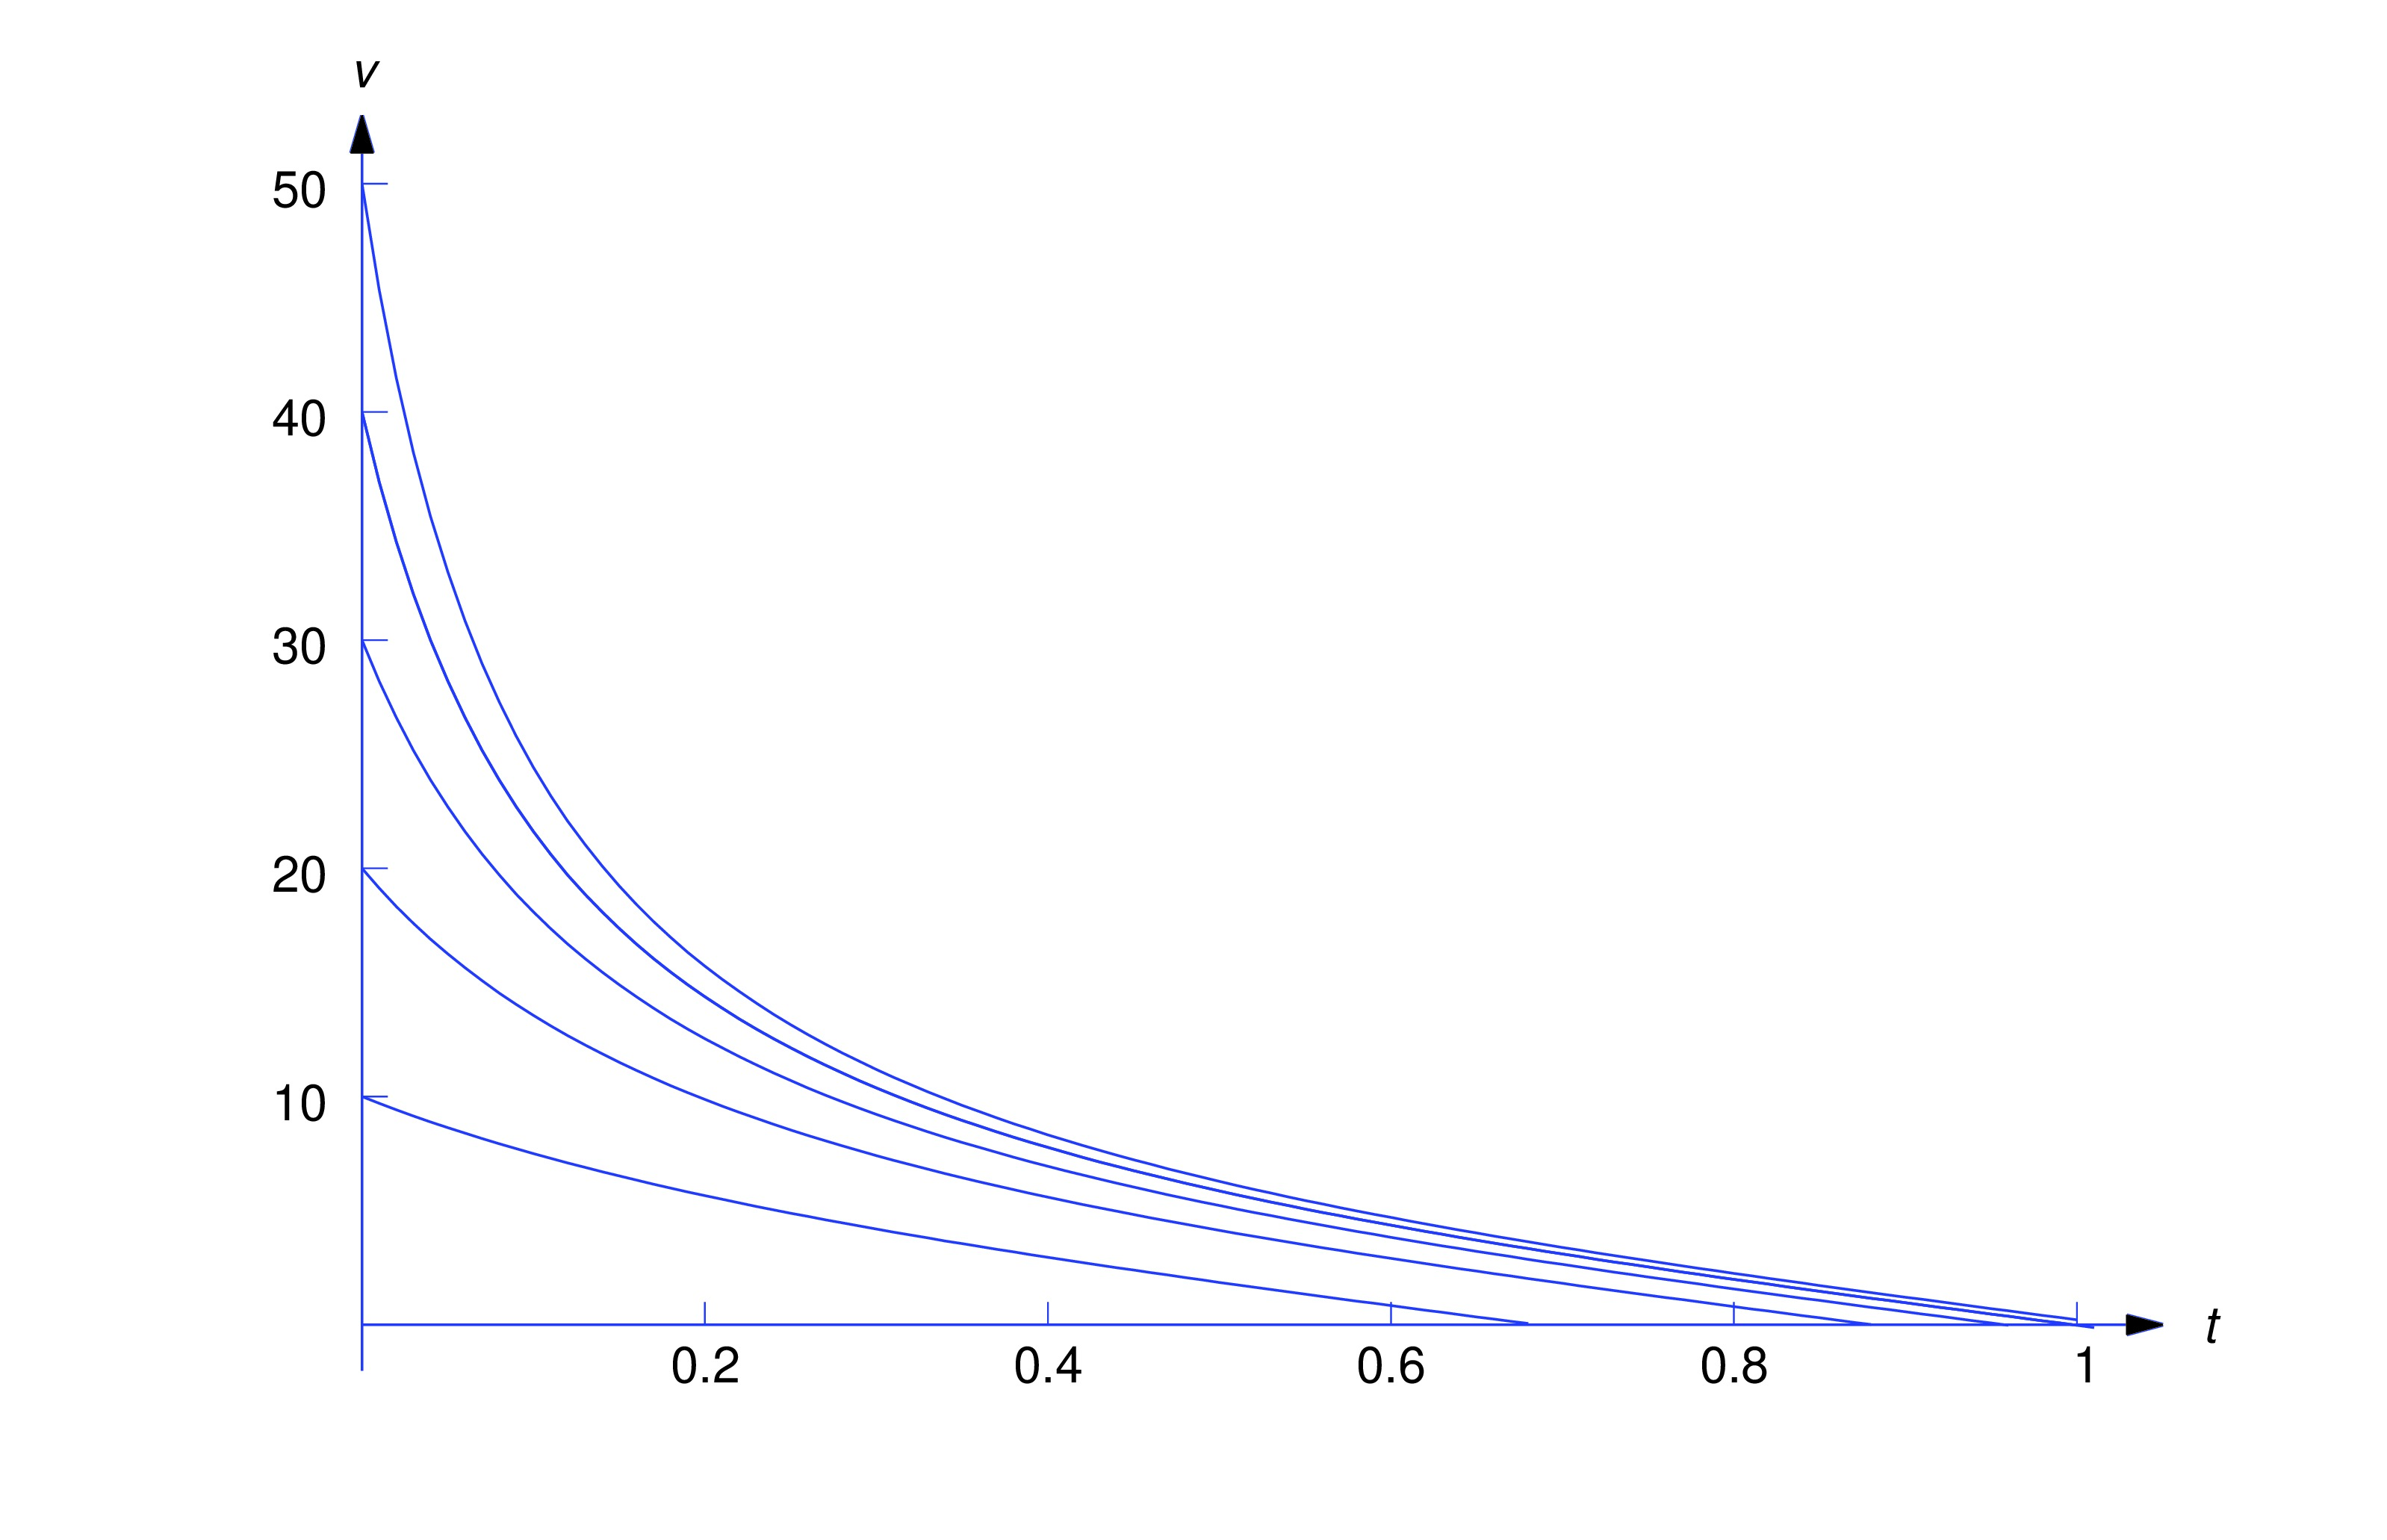
\includegraphics[height=1.5in]{fig040304.jpg} 
\end{image}
\end{explanation}
\end{example}

\subsection*{Escape Velocity}

Suppose a space vehicle is launched vertically and its fuel is
exhausted when the vehicle reaches an altitude $h$ above Earth, where
$h$ is sufficiently large so that resistance due to Earth's atmosphere
can be neglected. Let $t=0$ be the time when burnout occurs.
Assuming that the gravitational forces of all other celestial bodies
can be neglected, the motion of the vehicle for $t > 0$ is that of an
object with constant mass $m$ under the influence of Earth's
gravitational force, which we now assume to vary inversely with the
square of the distance from Earth's center;  thus, if we take the
upward direction to be positive then
gravitational force on the vehicle at an altitude $y$ above Earth is
\begin{equation} \label{eq:4.3.18}
F=-\frac{K}{(y+R)^2},
\end{equation}
where $R$ is  Earth's radius (see figure below).

\begin{image}
  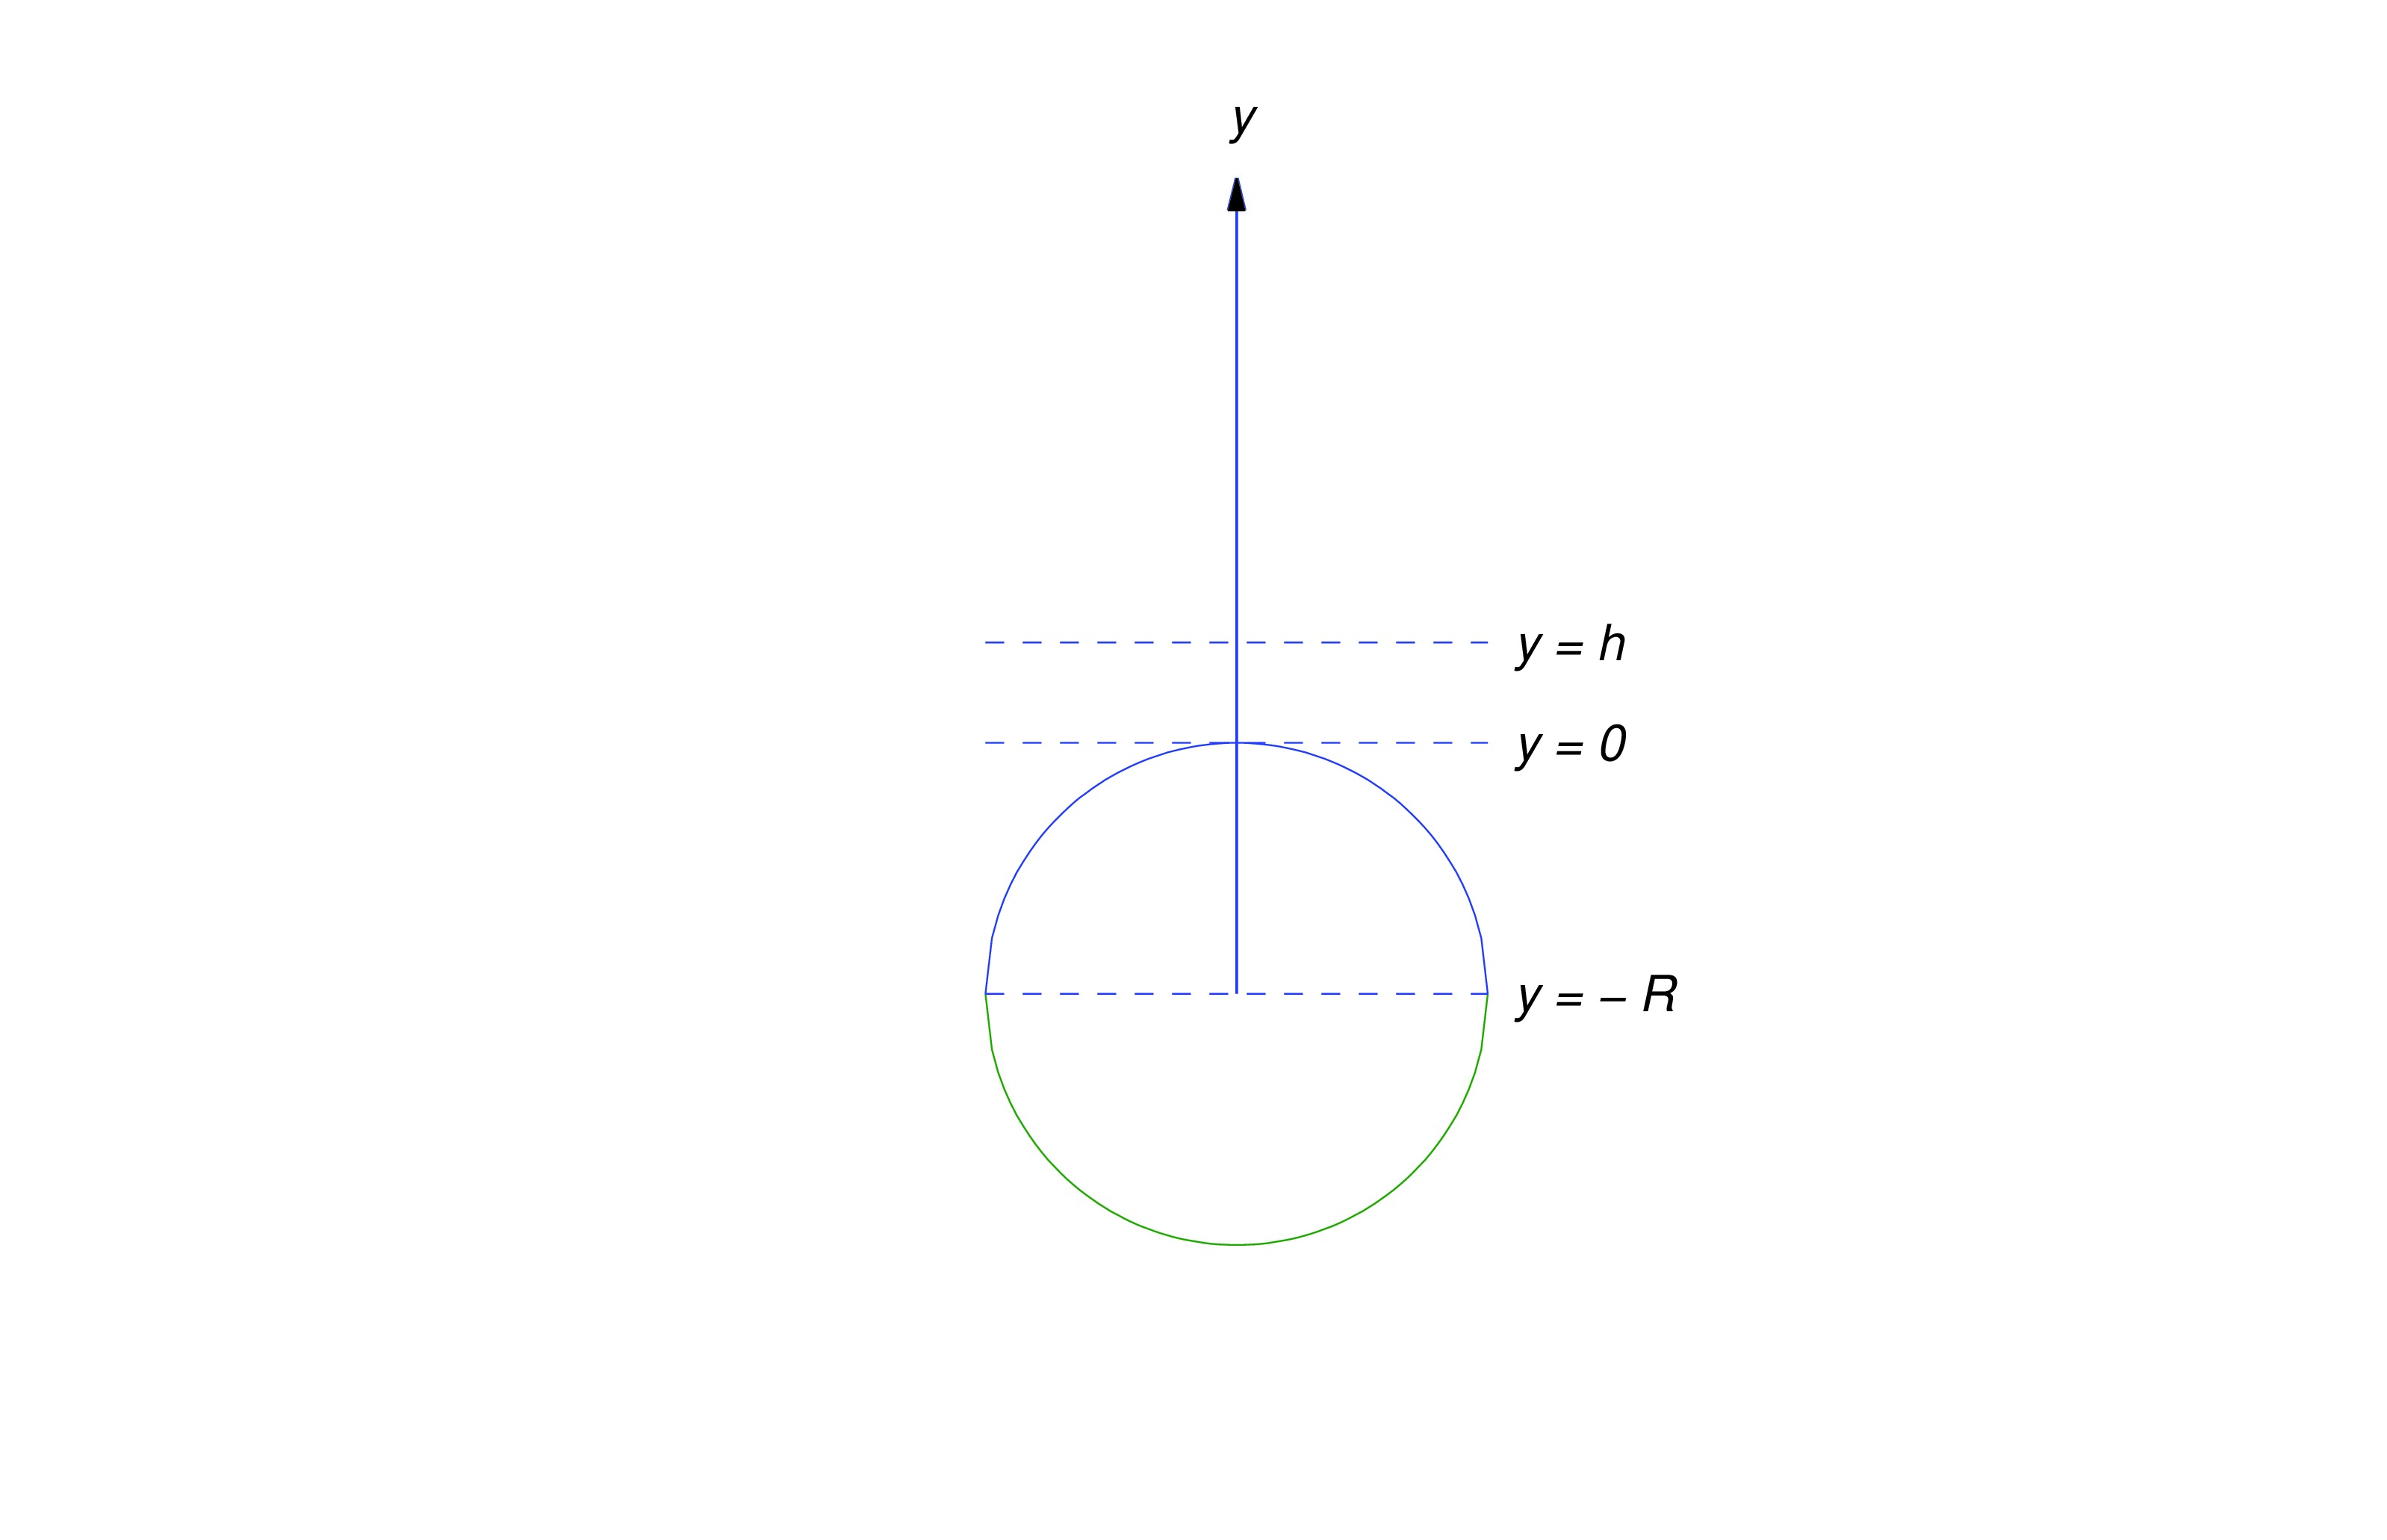
\includegraphics[height=1.5in]{fig040305.jpg} 
\end{image}

 Since $F=-mg$ when $y=0$, setting $y=0$ in
(\ref{eq:4.3.18}) yields
$$
-mg=-\frac{K}{R^2};
$$
 therefore $K=mgR^2$ and (\ref{eq:4.3.18}) can be written more
specifically as
\begin{equation} \label{eq:4.3.19}
F=-\frac{mgR^2}{(y+R)^2}.
\end{equation}

From Newton's second law of motion,
$$
F=m\frac{d^2y}{dt^2},
$$
so (\ref{eq:4.3.19}) implies that
\begin{equation} \label{eq:4.3.20}
\frac{d^2y}{dt^2}=-\frac{gR^2}{(y+R)^2}.
\end{equation}

We'll show that there's a number $v_e$, called the \textit{escape
velocity}, with these properties:

\begin{enumerate}
\item If $v_0\geq v_e$ then $v(t)>0$ for all $t>0$, and the vehicle
continues to climb for all $t>0$; that is, it ``escapes'' Earth.
(Is it really so obvious that $\lim_{t\rightarrow\infty}y(t)=\infty$
in this case?)
\item  If $v_0<v_e$  then  $v(t)$   decreases to zero and becomes negative.
Therefore
 the vehicle attains a  maximum
altitude  $y_m$ and
falls back to Earth.
 \end{enumerate}

Since
(\ref{eq:4.3.20}) is second order, we can't solve it by methods discussed
so far. However, we're concerned with $v$ rather than $y$, and $v$ is
easier to find. Since $v=y'$ the chain rule implies that
$$
\frac{d^2y}{dt^2}=\frac{dv}{dt}=\frac{dv}{dy}\frac{dy}{dt}=v\frac{dv}{dy}.
$$
 Substituting this into (\ref{eq:4.3.20}) yields the first order
separable equation
\begin{equation} \label{eq:4.3.21}
v\frac{dv}{dy}=-\frac{gR^2}{(y+R)^2}.
\end{equation}
When $t=0$, the velocity is $v_0$ and the altitude is $h$. Therefore
we can
obtain $v$ as a function of $y$ by solving the initial value problem
$$
v\frac{dv}{dy}=-\frac{gR^2}{(y+R)^2},\quad  v(h)=v_0.
$$

Integrating (\ref{eq:4.3.21}) with respect to $y$ yields
\begin{equation} \label{eq:4.3.22}
\frac{v^2}{2}=\frac{gR^2}{y+R}+c.
\end{equation}
 Since $v(h)=v_0$,
$$
c=\frac{v_0^2}{2}-\frac{gR^2}{h+R},
$$
 so (\ref{eq:4.3.22}) becomes
\begin{equation} \label{eq:4.3.23}
\frac{v^2}{2}=\frac{gR^2}{y+R}+\left(\frac{v_0^2}{2}-
\frac{gR^2}{h+R}\right).
\end{equation}
If
$$
v_0 \geq\left(\frac{2gR^2}{h+R}\right)^{1/2},
$$
 the parenthetical expression in (\ref{eq:4.3.23})  is nonnegative,
 so $v(y)>0$ for $y>h$. This proves that there's an escape
velocity $v_e$. We'll now prove that
$$
v_e=\left(\frac{2gR^2}{h+R}\right)^{1/2}
$$
by showing that the vehicle falls back to Earth if
\begin{equation} \label{eq:4.3.24}
v_0 <\left(\frac{2gR^2}{h+R}\right)^{1/2}.
\end{equation}
If (\ref{eq:4.3.24})  holds then  the parenthetical expression in
(\ref{eq:4.3.23})
is negative and the vehicle will attain a maximum altitude $y_m>h$
that satisfies the equation
$$
0=\frac{gR^2}{y_m+R}+\left(\frac{v_0^2}{2}-
\frac{gR^2}{h+R}\right).
$$
The velocity will be zero at the maximum  altitude, and the object will
then fall to Earth under the influence of gravity.


\section*{Text Source}
Trench, William F., "Elementary Differential Equations" (2013). Faculty Authored and Edited Books \& CDs. 8. (CC-BY-NC-SA)

\href{https://digitalcommons.trinity.edu/mono/8/}{https://digitalcommons.trinity.edu/mono/8/}


\end{document}